\chapter{Spontane Supersymmetriebrechung und das erste \texorpdfstring{\(SU(5)\)}{SU(5)}-Multiplett}

\lectureoverview{Symmetriebrechung zeigt sich hier zunächst als unmittelbar erkennbare Eigenschaft der Spektren: Ein rotationsinvariantes Atom hat entartete Drehimpulsniveaus, während ein Magnetfeld sie aufspaltet. Ein Ferromagnet vermittelt dann die subtilere Einsicht, dass die Gleichungen eine Symmetrie bewahren können, die das Vakuum nicht besitzt. Lückenlose Magnonen, die Bedingung \(J|0\rangle\neq0\) und ein von null verschiedener Ordnungsparameter sind drei Beschreibungen desselben Phänomens. Wir übertragen dieses Muster auf eine chirale supersymmetrische Feldtheorie, leiten das skalare Potential \(V=|W'|^2\) her, indem wir das Hilfsfeld \(F\) eliminieren, und unterscheiden supersymmetrische von durch \(F\)-Brechung gekennzeichneten Vakua. Die daraus folgende Vakuumenergie, die Aufspaltung zwischen Bosonen--und Fermionen, das Goldstino, der verborgene Sektor und der Super-Higgs-Mechanismus schließen die Diskussion der Supersymmetrie ab. Im letzten Teil wechseln wir das Thema und wenden uns der großen Vereinheitlichung zu: \(SU(3)\times SU(2)\times U(1)\) wird blockweise in \(SU(5)\) eingebettet, dessen erstes Materiemultiplett ein Leptondublett mit drei Anti-Down-Quarks vereint.}

\section{Ein Spektrum bewahrt die Erinnerung an seine Symmetrie}

Der Grund, mit einem Atom zu beginnen, ist nicht bloß, die elementare Quantenmechanik zu wiederholen. Energieniveaus und Teilchenmassen sind dieselbe Art von Spektraldaten. Wenn eine Symmetrie atomare Energieniveaus zur Entartung zwingt, kann ihre Brechung diese Niveaus aufspalten; in der Feldtheorie bedeutet dies entsprechend, dass Mitglieder eines Teilchenmultipletts unterschiedliche Massen annehmen können.

Ein Atomzustand habe den Gesamtdrehimpuls \(j\), der sowohl Spin- als auch Bahnbeiträge umfasst. Bezüglich einer beliebig gewählten Achse gilt
\begin{equation}
J_z|j,m\rangle=m\hbar|j,m\rangle,
\qquad
m=-j,-j+1,\ldots,j,
\end{equation}
also gibt es \(2j+1\) Zustände. Die vertrauten Pfeile in Lehrbüchern sollte man nicht so verstehen, als hätte der Drehimpulsvektor tatsächlich nur \(2j+1\) mögliche räumliche Richtungen. Quantisiert ist seine Komponente entlang der gewählten Achse.

Im leeren, rotationsinvarianten Raum gibt es keinen physikalischen Grund, diese Achse auszuzeichnen. Eine Rotation mischt die Zustände innerhalb des Spin-\(j\)-Multipletts, und die Invarianz des Hamiltonoperators impliziert
\begin{equation}
[H,\mathbf J]=0,
\qquad
E_{j,-j}=E_{j,-j+1}=\cdots=E_{j,j}.
\label{eq:l9-degeneracy}
\end{equation}

\begin{classroomqa}
\audiencequestion{Welche Symmetrie besagt, dass eine Drehung des gesamten Atoms seine Energie nicht ändern kann? \lecturetimestamp{00:05:53}}
\lecturerresponse{Rotationssymmetrie. Da eine Rotation eine Orientierung des Drehimpulses in eine andere überführt, ohne das physikalische System zu verändern, haben alle \(2j+1\) Zustände dieselbe Energie.}
\end{classroomqa}

Legt man nun ein Magnetfeld \(\mathbf B=B\hat{\mathbf z}\) an, so unterscheidet die Wechselwirkung
\begin{equation}
H_B=-\boldsymbol{\mu}\cdot\mathbf B
\end{equation}
die Komponente parallel zum Feld. Schematisch gilt:
\begin{equation}
\Delta E_m\propto mB.
\label{eq:l9-zeeman}
\end{equation}
Bei schwachem Feld spalten sich Niveaus mit unterschiedlichem \(m\) linear auf, und Übergänge zwischen ihnen spalten Spektrallinien auf.

\begin{classroomqa}
\audiencequestion{Wie nennt man die Aufspaltung atomarer Energieniveaus in einem Magnetfeld? \lecturetimestamp{00:07:13}}
\lecturerresponse{Den Zeeman-Effekt. Er ist das Musterbeispiel für die gesamte folgende Diskussion: Durch eine Symmetrie entartete Niveaus spalten sich auf, wenn ein Hintergrundfeld diese Symmetrie bricht.}
\end{classroomqa}

\begin{center}
\begin{tikzpicture}[x=1.05cm,y=0.75cm,>=Latex]
  \draw[thick] (-3,0) -- (-1,0);
  \node[left] at (-3,0) {\(B=0\)};
  \foreach \y/\m in {-1.2/-1,-0.4/0,0.4/1,1.2/2} {
    \draw[thick,teal!70!black] (1,\y) -- (3,\y);
    \node[right] at (3,\y) {\(m=\m\)};
  }
  \draw[->,thick] (-0.5,0) -- (0.6,0);
  \node[above] at (0.05,0) {\(\mathbf B\neq0\)};
\end{tikzpicture}
\end{center}

\section{Der Ferromagnet: symmetrische Gesetze, asymmetrisches Vakuum}

Ein einfaches mikroskopisches Modell eines Ferromagneten ordnet jedem Gitterplatz ein kleines magnetisches Moment zu. Senken benachbarte Momente ihre Energie, indem sie sich parallel ausrichten, ist die Tieftemperaturphase ferromagnetisch. Wird eine antiparallele Ausrichtung bevorzugt, entsteht ein Antiferromagnet. Starke thermische oder quantenmechanische Fluktuationen können dagegen eine Nettomagnetisierung vollständig auslöschen.

Angenommen, ein Ferromagnet erfüllt die ganze Welt und nimmt einen gleichmäßig ausgerichteten Zustand an. Sein internes Magnetfeld spaltet die Energieniveaus eines Atoms ebenso auf wie ein von außen angelegtes Feld. Es gibt jedoch einen entscheidenden Unterschied. Die zugrunde liegenden Wechselwirkungen bevorzugen weder Norden noch Osten noch irgendeine andere Richtung. Jede gleichmäßig gedrehte Konfiguration hat dieselbe Energie:
\begin{equation}
\mathbf M(\mathbf x)=M_0\hat{\mathbf n},
\qquad
\hat{\mathbf n}\in S^2.
\label{eq:l9-ferromagnetic-vacua}
\end{equation}
Die Gleichungen sind rotationsinvariant, aber ein tatsächlicher Grundzustand wählt eine bestimmte Richtung \(\hat{\mathbf n}\) aus. Die Symmetriebrechung ist spontan und nicht explizit.

Ein Bewohner, der aus Anregungen dieses Mediums besteht, kann nicht das ganze Universum ergreifen und drehen. Lokal erscheint die gewählte Richtung daher ebenso grundlegend wie ein äußeres Feld. Ein Atom beobachtet weiterhin dasselbe Niveauschema; sein Drehimpuls ist dabei entlang \(\hat{\mathbf n}\) statt entlang einer von außen festgelegten \(z\)-Achse aufgelöst. Die Frage ist, wie ein interner Beobachter herausfinden könnte, dass die scheinbare Asymmetrie zum Zustand und nicht zu den Gesetzen gehört.

\subsection{Das Goldstone-Kriterium}

Eine gleichmäßige Drehung aller Momente führt von einem Vakuum in Gl.~\eqref{eq:l9-ferromagnetic-vacua} zu einem anderen und kostet keine Energie. Ändert sich die Orientierung stattdessen sehr allmählich im Raum, ziehen benachbarte Momente aneinander, und die Verzerrung breitet sich als Spinwelle aus, deren Quanten Magnonen sind. Für gegen unendlich gehende Wellenlänge nähert sich die Konfiguration einer gleichmäßigen Drehung an, sodass ihre Anregungsenergie gegen null geht:
\begin{equation}
k=\frac{2\pi}{\lambda}\longrightarrow0
\quad\Longrightarrow\quad
E(k)\longrightarrow0.
\label{eq:l9-gapless-magnon}
\end{equation}
Zwei Bewohner können benachbarte Momente zum Schwingen bringen, solche Wellen durch das Medium schicken und ihre beliebig kleine Energie messen. Dieses Experiment weist die spontane Brechung nach, obwohl sie die Welt nicht drehen können.

\editorialnote{Ein ferromagnetisches Magnon ist lückenlos, hat aber im Allgemeinen eine nichtrelativistische quadratische Dispersionsrelation \(E\propto k^2\) statt der relativistischen Beziehung \(E\propto|k|\). In der Vorlesung wird der Begriff masselos im physikalisch relevanten Sinn einer verschwindenden Lücke verwendet. Beide sind Goldstone-Moden.}

Dieselbe Idee gilt für kontinuierliche innere Symmetrien, darunter die Eich- und Flavourgruppen der Teilchenphysik. Ist die gebrochene Symmetrie jedoch lokal geeicht, bleibt die Goldstone-Mode nicht als unabhängiges masseloses Teilchen erhalten.

\begin{classroomqa}
\audiencequestion{Was geschieht, wenn spontane Symmetriebrechung mit Eichinvarianz zusammentrifft? \lecturetimestamp{00:15:56}}
\lecturerresponse{Das Goldstone-Boson liefert dem Eichfeld eine zusätzliche Polarisation. Das Eichboson wird massiv; dies ist der Higgs-Mechanismus, auf den wir in der Gravitationsanalogie zurückkommen werden.}
\end{classroomqa}

\section{Drei gleichwertige Anzeichen der Symmetriebrechung}

Der Ferromagnet lässt sich nun in drei einander ergänzenden Sprachen beschreiben.

\paragraph{Entartete Vakua.}
Für jede Orientierung \(\hat{\mathbf n}\) gibt es einen Zustand minimaler Energie. Die Physik findet in einem ausgewählten Zustand dieser Familie statt, obwohl die Symmetrie alle Zustände miteinander verknüpft.

\paragraph{Ein Generator, der das Vakuum nicht annihiliert.}
Sei \(J_a\) ein Generator von Drehungen. Eine endliche Transformation lautet
\begin{equation}
U(\epsilon)=e^{-i\epsilon J_a},
\end{equation}
und \(J_a|0\rangle\) ist proportional zur infinitesimalen Änderung des Vakuums, nicht zum gesamten gedrehten Zustand.

\begin{classroomqa}
\audiencequestion{Was sind die Generatoren der Rotationssymmetrie? \lecturetimestamp{00:17:29}}
\lecturerresponse{Die Komponenten des Gesamtdrehimpulses. Wir bezeichnen sie mit \(J_a\), weil sie alles im Zustand drehen und nicht nur ein einzelnes Atom.}
\end{classroomqa}

Für einen ungebrochenen Generator gilt
\begin{equation}
J_a|0\rangle=0.
\label{eq:l9-unbroken-generator}
\end{equation}
Ein gebrochener Generator ergibt dagegen
\begin{equation}
J_a|0\rangle\neq0.
\label{eq:l9-broken-generator}
\end{equation}

\begin{classroomqa}
\audiencequestion{Ergibt \(J_a|0\rangle\) bei einem Wert ungleich null einfach dasselbe Vakuum? \lecturetimestamp{00:19:43}}
\lecturerresponse{Nein. Es ergibt die infinitesimale Differenz zwischen dem gewählten Vakuum und einem leicht gedrehten Vakuum. Physikalisch entspricht diese Differenz einer Goldstone-Anregung mit unendlich großer Wellenlänge.}
\end{classroomqa}

\begin{classroomqa}
\audiencequestion{Ändert diese infinitesimale Drehung die Energie? \lecturetimestamp{00:20:14}}
\lecturerresponse{Nein. Das gedrehte Vakuum ist gegenüber dem ursprünglichen entartet, daher hat der Goldstone-Zustand mit verschwindendem Impuls Energie null.}
\end{classroomqa}

Symbolisch gilt
\begin{equation}
J_a|0\rangle
\sim
|\pi_a,\mathbf k=0\rangle,
\label{eq:l9-generator-goldstone}
\end{equation}
wobei \(\pi_a\) die Goldstone-Mode bezeichnet, die dem gebrochenen Generator entspricht.

\paragraph{Ein von null verschiedener Ordnungsparameter.}
Die lokale Magnetisierung \(\mathbf M(\mathbf x)\) ist ein Feld. In einer warmen oder quantenmechanisch ungeordneten Phase gilt
\begin{equation}
\langle\mathbf M\rangle=0,
\end{equation}
und das Vakuum zeichnet keine Richtung aus. In der geordneten Phase gilt
\begin{equation}
\langle M_i\rangle\neq0
\quad\text{for at least one component }i,
\label{eq:l9-magnetization-order}
\end{equation}
sodass eine Drehung diese von null verschiedene Komponente in die übrigen mischt. Entartete Vakua, ein gebrochener Generator und ein von null verschiedener Ordnungsparameter sind die drei Muster, die wir auf die Supersymmetrie übertragen.

\section{Das chirale Multiplett: Wiederholung}

Das einfachste vierdimensionale Beispiel enthält ein komplexes skalares Feld, ein Weyl-Fermion und ein komplexes Hilfsskalarenfeld. In chiralen Koordinaten gilt
\begin{equation}
y^\mu=x^\mu+i\bar\theta\bar\sigma^\mu\theta,
\end{equation}
und ein chirales Superfeld lässt sich schematisch entwickeln als
\begin{equation}
\Phi(y,\theta)=
\phi(y)+\sqrt2\,\theta\psi(y)+\theta^2F(y).
\label{eq:l9-chiral-expansion}
\end{equation}
In der Vorlesung wird der konventionelle Faktor \(\sqrt2\) weggelassen; von nun an nehmen wir ihn auf, damit die Koeffizienten der Komponenten der Standardkonvention entsprechen. Ein chirales Superfeld ist von sich aus komplex: Eine Realitätsbedingung bleibt unter seiner Supersymmetrietransformation nicht erhalten.

Die supersymmetrische kinetische Wirkung lautet
\begin{equation}
S_{\mathrm{kin}}
=
\int d^4x\,d^4\theta\,
\Phi^\dagger\Phi.
\label{eq:l9-kahler-action}
\end{equation}
Die Grassmann-Integration wählt den Koeffizienten von
\(\theta^2\bar\theta^2\) aus. Bei einer Metrik mit Signatur überwiegend minus ergibt sich für die Komponenten
\begin{equation}
\mathcal L_{\mathrm{kin}}
=
\partial_\mu\phi^\ast\,\partial^\mu\phi
+i\bar\psi\bar\sigma^\mu\partial_\mu\psi
+F^\ast F.
\label{eq:l9-chiral-kinetic}
\end{equation}
Die ersten beiden Terme beschreiben die Ausbreitung des Skalarfelds und des Fermions. Der letzte Term enthält keine Ableitung und beschreibt daher kein sich ausbreitendes Teilchen.

\begin{figure}[H]\centering
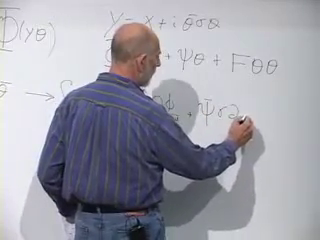
\includegraphics[width=0.76\textwidth]{lecture_09_figure_02.png}\lectureframe{00:27:36.000}\caption{Die chirale Koordinate und die Komponentenentwicklung über den Skalar-, Fermion- und Hilfsfeldterm.}\end{figure}

\section{Was das \texorpdfstring{\(d^2\theta\)}{d2-Theta}-Integral auswählt}

Wechselwirkungen und Massen entstehen aus einer holomorphen Funktion \(W(\Phi)\), dem Superpotential:
\begin{equation}
S_W
=
\int d^4x
\left[
\int d^2\theta\,W(\Phi)
+\mathrm{h.c.}
\right].
\label{eq:l9-superpotential-action}
\end{equation}
Ein chiraler Ausdruck hängt nicht unabhängig von \(\bar\theta\) ab; deshalb wäre sein Integral über alle vier ungeraden Koordinaten null. Das Integral über \(d^2\theta\) wählt stattdessen seine \(\theta^2\)-Komponente aus.

Um die Kombinatorik zu erkennen, bevor wir eine allgemeine Funktion betrachten, sei \(W(\Phi)=\Phi^n\). In
\begin{equation}
(\phi+\sqrt2\,\theta\psi+\theta^2F)^n,
\end{equation}
gibt es zwei Möglichkeiten, genau zwei \(\theta\) zu erhalten: Man kann ein einzelnes \(F\theta^2\) auswählen oder zwei fermionische Faktoren.

\begin{classroomqa}
\audiencequestion{Wie viele Terme enthalten ein ausgewähltes \(F\theta^2\) und ansonsten nur Skalarfelder: \(n-1\) oder \(n\)? \lecturetimestamp{00:31:33}}
\lecturerresponse{Es gibt \(n\). Jeder der \(n\) Faktoren kann \(F\theta^2\) liefern; die übrigen \(n-1\) Faktoren liefern \(\phi\). Der Beitrag ist \(nF\phi^{n-1}\).}
\end{classroomqa}

\begin{classroomqa}
\audiencequestion{Auf wie viele Arten können zwei Faktoren die beiden Fermionen liefern? \lecturetimestamp{00:32:26}}
\lecturerresponse{Es gibt \(\binom n2=n(n-1)/2\) ungeordnete Auswahlmöglichkeiten. Die Grassmann-Kontraktion legt den entsprechenden Term \(\psi\psi\) fest.}
\end{classroomqa}

In der Notation der Vorlesung, in der Koeffizienten unterdrückt werden, ergibt sich also
\begin{equation}
\int d^2\theta\,\Phi^n+\mathrm{h.c.}
\;\leadsto\;
nF\phi^{n-1}
-\frac{n(n-1)}{2}\phi^{n-2}\psi\psi
+\mathrm{h.c.}
\label{eq:l9-power-extraction}
\end{equation}
Das hier angegebene Minuszeichen folgt aus der standardmäßigen normierten Entwicklung und der Grassmann-Konvention; bei einem Wechsel der Konvention können sich oberflächliche Vorzeichen ändern.

\begin{classroomqa}
\audiencequestion{Was geschah mit dem Term \(\phi^n\), der gar keine \(\theta\) enthält? \lecturetimestamp{00:33:10}}
\lecturerresponse{Er ist im Produkt enthalten, wird aber von \(d^2\theta\) verworfen. Der Pfeil bedeutet, dass die Integration den Koeffizienten von \(\theta^2\) auswählt; er bedeutet nicht, dass die vollständigen Ausdrücke gleich sind.}
\end{classroomqa}

\begin{figure}[H]\centering
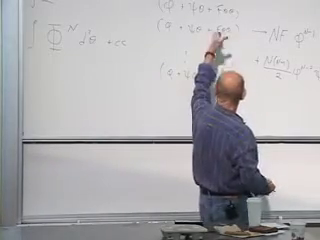
\includegraphics[width=0.82\textwidth]{lecture_09_figure_03.png}\lectureframe{00:33:38.000}\caption{Die wiederholten Superfeldfaktoren und der Implikationspfeil, der die Komponente mit zwei \(\theta\) herausgreift, statt sie mit dem Ausdruck gleichzusetzen.}\end{figure}

Fasst man Potenzen mit beliebigen Koeffizienten zusammen, werden die kombinatorischen Faktoren zu Ableitungen:
\begin{equation}
\int d^2\theta\,W(\Phi)+\mathrm{h.c.}
\;\leadsto\;
F W'(\phi)
-\frac12 W''(\phi)\psi\psi
+\mathrm{h.c.}
\label{eq:l9-W-components}
\end{equation}

\begin{classroomqa}
\audiencequestion{Warum enthält der Fermionterm \(\phi^{n-2}\) statt \(\phi^{n-1}\)? \lecturetimestamp{00:36:32}}
\lecturerresponse{Zwei Faktoren haben bereits die Fermionen geliefert, sodass \(n-2\) Skalarfaktoren übrig bleiben. Der Koeffizient ist die Hälfte der zweiten Ableitung \(W''(\phi)\).}
\end{classroomqa}

Der Fermionterm ist wichtig: Er ergibt eine Masse, wenn \(W''\) konstant ist, und eine Yukawa-Wechselwirkung, wenn \(W''\) von \(\phi\) abhängt. Für die Vakuumanalyse enthält jedoch der Hilfsfeldterm \(FW'\) die unmittelbar relevante Information.

\section{Elimination des Hilfsfelds}

Fassen wir die Terme zusammen, die \(F\) enthalten:
\begin{equation}
\mathcal L_F
=
F^\ast F
+F W'(\phi)
+F^\ast \overline{W'(\phi)}.
\label{eq:l9-LF}
\end{equation}
Da es keinen Term mit \(\partial_\mu F\) gibt, reduziert sich die vollständige Euler--Lagrange-Gleichung
\begin{equation}
\partial_\mu
\frac{\partial\mathcal L}{\partial(\partial_\mu F)}
-
\frac{\partial\mathcal L}{\partial F}
=0
\end{equation}
unmittelbar auf eine algebraische Gleichung. Behandelt man \(F\) und \(F^\ast\) als unabhängige Variablen, erhält man
\begin{align}
\frac{\partial\mathcal L_F}{\partial F}
&=F^\ast+W'(\phi)=0,
&
\frac{\partial\mathcal L_F}{\partial F^\ast}
&=F+\overline{W'(\phi)}=0,
\label{eq:l9-F-eom}
\end{align}
und damit
\begin{equation}
F^\ast=-W'(\phi),
\qquad
F=-\overline{W'(\phi)}.
\label{eq:l9-F-solution}
\end{equation}

\begin{figure}[H]\centering
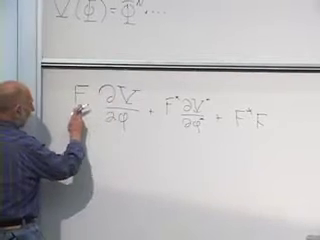
\includegraphics[width=0.82\textwidth]{lecture_09_figure_04.png}\lectureframe{00:39:40.000}\caption{Der vollständige Ausdruck für das Hilfsfeld und seine algebraische Bewegungsgleichung sind gemeinsam zu sehen, nachdem die Sicht auf die Tafel freigegeben wurde.}\end{figure}

\begin{classroomqa}
\audiencequestion{Müsste diese Ableitung nach \(\phi\) genommen werden statt nach dem an der Tafel notierten konjugierten Feld? \lecturetimestamp{00:41:21}}
\lecturerresponse{Ja. Die Korrektur stellt das konjugierte Paar in Gl.~\eqref{eq:l9-F-eom} wieder her: \(F^\ast=-W'(\phi)\) und \(F=-\overline{W'(\phi)}\).}
\end{classroomqa}

Einsetzen in Gl.~\eqref{eq:l9-LF} ergibt
\begin{equation}
\mathcal L_F\big|_{\mathrm{on\ shell}}
=-|W'(\phi)|^2.
\end{equation}
Da eine skalare Lagrange-Dichte die Form kinetische Energie minus potentielle Energie hat, lautet das gewöhnliche skalare Potential
\begin{equation}
\boxed{V(\phi,\phi^\ast)=|W'(\phi)|^2\ge0.}
\label{eq:l9-F-potential}
\end{equation}
Dieses \(V\) ist nicht das Superpotential. Wir verwenden \(W\) für die holomorphe Funktion im Superspace und \(V\) für die gewöhnliche potentielle Energie.

\subsection{Zwei unmittelbare Beispiele}

Bei exakten Standardnormierungen gilt
\begin{equation}
\begin{gathered}
W(\Phi)=\frac12m\Phi^2,\\
W'(\phi)=m\phi,
\qquad V=|m|^2|\phi|^2.
\end{gathered}
\label{eq:l9-quadratic-W}
\end{equation}
Derselbe Term ergibt die Fermionmasse
\(-\tfrac12m\psi\psi+\mathrm{h.c.}\), sodass die Massen von Skalar und Fermion vor der Supersymmetriebrechung übereinstimmen.

Für
\begin{equation}
W(\Phi)=\frac{g}{3}\Phi^3,
\end{equation}
erhält man
\begin{equation}
\begin{gathered}
W'(\phi)=g\phi^2,
\qquad V=|g|^2|\phi|^4,\\
\mathcal L_{\mathrm{Yukawa}}
=-g\phi\psi\psi+\mathrm{h.c.}
\end{gathered}
\label{eq:l9-cubic-W}
\end{equation}
Der quartische Skalarvertex beschreibt die Streuung zweier Skalarteilchen, während der Yukawa-Term der zugehörige supersymmetrische Partner ist.

\section{Zwei Arten von Vakuum}

Das Vakuum ist eine konstante Feldkonfiguration an einem Minimum von \(V\); die Ableitungsterme verschwinden. Da Gl.~\eqref{eq:l9-F-potential} nichtnegativ ist, sind zwei Fälle möglich.

\subsection{Ein Minimum mit verschwindender Energie}

Erfüllt ein \(\phi_0\) die Bedingung
\begin{equation}
W'(\phi_0)=0,
\end{equation}
so gilt
\begin{equation}
V(\phi_0)=0,
\qquad
\langle F\rangle=0.
\label{eq:l9-unbroken-F}
\end{equation}
Das Vakuum ist supersymmetrisch. Es entspricht der verschwindenden Magnetisierung: Keine Hilfskomponente hat eine Richtung im Superspace ausgewählt.

\subsection{Ein angehobenes Minimum}

Haben die Gleichungen
\begin{equation}
W'(\phi)=0
\label{eq:l9-F-flatness}
\end{equation}
am Minimum keine gemeinsame Lösung, so gilt
\begin{equation}
V_{\min}>0,
\qquad
\langle F\rangle\neq0,
\label{eq:l9-broken-F}
\end{equation}
und die Supersymmetrie ist spontan gebrochen. Die Wirkung bleibt supersymmetrisch, ihr Zustand niedrigster Energie jedoch nicht.

\begin{figure}[H]\centering
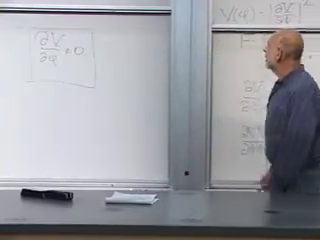
\includegraphics[width=0.88\textwidth]{lecture_09_figure_05.png}\lectureframe{00:52:09.960}\caption{Die Tafel zeigt weiterhin das positive Potential, die \(F\)-Gleichung und die Vakuumbedingung und macht zugleich den Unterschied zwischen symmetrischen Gleichungen und einer nicht symmetrischen Lösung deutlich.}\end{figure}

Die Aussage über den Ordnungsparameter lässt sich anhand der Fermiontransformation präzisieren:
\begin{equation}
\delta\psi_\alpha
=
i\sqrt2
(\sigma^\mu\bar\epsilon)_\alpha\partial_\mu\phi
+\sqrt2\,\epsilon_\alpha F.
\label{eq:l9-fermion-transformation}
\end{equation}
Bei einem homogenen Vakuum verschwindet der Ableitungsterm. Falls
\(\langle F\rangle\neq0\), verschiebt die Supersymmetrie das Fermion um eine von null verschiedene Konstante, sodass das Vakuum invariant sein kann.\editorialnote{Gleichung~\eqref{eq:l9-fermion-transformation} ist die übliche Komponentenform, die explizit zeigt, dass sich die Komponenten eines Superfelds ineinander transformieren.}

Dasselbe Ergebnis folgt aus der Superalgebra. Im Ruhesystem gilt
\begin{equation}
\{Q_\alpha,Q_{\dot\alpha}^\dagger\}
=2\sigma^0_{\alpha\dot\alpha}H.
\end{equation}
Der Erwartungswert im Vakuum drückt seine Energie als Summe der Normen der Superladungen aus, die auf das Vakuum wirken:
\begin{equation}
E_0\ge0,
\qquad
E_0=0
\ \Longleftrightarrow\
Q_\alpha|0\rangle
=Q_{\dot\alpha}^\dagger|0\rangle=0.
\label{eq:l9-algebra-vacuum-energy}
\end{equation}
Somit sind positive Vakuumenergie und spontane Supersymmetriebrechung zwei Seiten derselben Aussage über starre Supersymmetrie.

\begin{center}
\begin{tikzpicture}[x=1.2cm,y=1.0cm,>=Latex]
  \draw[->] (-3,0) -- (-0.2,0) node[right] {\(\phi\)};
  \draw[->] (-2.8,-0.15) -- (-2.8,2.1) node[above] {\(V\)};
  \draw[thick,teal!75!black,domain=-2.5:-0.5,samples=60]
    plot (\x,{0.65*(\x+1.5)^2});
  \fill (-1.5,0) circle (2pt);
  \node[below] at (-1.5,0) {\(F=0\)};
  \draw[->] (0.4,0) -- (3.2,0) node[right] {\(\phi\)};
  \draw[->] (0.6,-0.15) -- (0.6,2.1) node[above] {\(V\)};
  \draw[thick,orange!85!black,domain=0.9:2.9,samples=60]
    plot (\x,{0.55*(\x-1.9)^2+0.65});
  \fill (1.9,0.65) circle (2pt);
  \draw[dashed] (0.6,0.65) -- (1.9,0.65);
  \node[below] at (1.9,0.65) {\(F\neq0\)};
\end{tikzpicture}
\end{center}

\editorialnote{Ein minimales Beispiel ist \(W=f\Phi\), wobei \(W'=f\) niemals verschwindet und \(V=|f|^2\) gilt. Dieses Ein-Feld-Beispiel hat eine flache skalare Richtung; realistische Brechung durch einen \(F\)-Term wird üblicherweise mit mehreren chiralen Feldern umgesetzt, etwa in verborgenen Sektoren vom O'Raifeartaigh-Typ.}

\section{Was eine gebrochene Supersymmetrie hervorbringt}

\subsection{Massenaufspaltung}

Die Analogie zum Ferromagneten wird nun wieder spektral. Ein schwaches internes Magnetfeld spaltet Atomniveaus auf, ohne die Identität des Atoms aufzuheben. Entsprechend spaltet ein schwach vermittelter Supersymmetriebrechungs-Ordnungsparameter Bosonen und Fermionen auf, die andernfalls zu einem Supermultiplett gehören würden.

\begin{classroomqa}
\audiencequestion{Welche Teilchen werden durch Supersymmetrie ineinander transformiert und verlieren deshalb ihre Massentartung, wenn das Vakuum sie bricht? \lecturetimestamp{00:51:40}}
\lecturerresponse{Bosonen und Fermionen. Ihre Massen müssen nicht länger übereinstimmen, sobald der Zustand die Transformation, die sie miteinander verknüpft, nicht mehr respektiert.}
\end{classroomqa}

Die Aufspaltung wird nicht allein durch \(\langle F\rangle\) verursacht; sie hängt von den Kopplungen ab, die die Brechung auf die sichtbaren Felder übertragen. Sind diese Kopplungen schwach, bleiben die sichtbaren Teilchen als solche erkennbar, und die Aufspaltungen sind klein gegenüber den Skalen der großen Vereinheitlichung oder der Planck-Skala. Wären die Kopplungen stark, entspräche dies einem Atom, das durch ein enorm starkes Magnetfeld so verzerrt wird, dass es sich zu einem langen, nicht wiedererkennbaren Objekt verformt.

\subsection{Das Goldstino}

Bei einem gewöhnlichen gebrochenen Generator erzeugt \(J|0\rangle\) einen bosonischen Goldstone-Zustand. Eine Superladung ist fermionisch und wandelt bosonische Zustände in fermionische um. Da das Vakuum als bosonisch gilt, erzeugt eine gebrochene Superladung einen fermionischen Zustand mit Energie null:
\begin{equation}
Q_\alpha|0\rangle
\sim
|\widetilde G_\alpha,\mathbf k=0\rangle.
\label{eq:l9-goldstino}
\end{equation}
Seine sich ausbreitende Anregung ist ein masseloses Weyl-Fermion, das Goldstone-Fermion oder Goldstino.

\begin{classroomqa}
\audiencequestion{Welchen neuen Zustand erzeugt eine Supersymmetrietransformation, die das Vakuum nicht invariant lässt? \lecturetimestamp{00:53:24}}
\lecturerresponse{Ein masseloses Fermion. Das gewöhnliche Goldstone-Theorem-Muster bleibt bestehen, doch ein fermionischer Generator verwandelt das bosonische Vakuum in das Goldstino.}
\end{classroomqa}

Spontane Supersymmetriebrechung in einer Theorie mit starrer Supersymmetrie hat daher zwei unvermeidliche Kennzeichen:
\begin{equation}
\boxed{
V_{\min}>0
\qquad\text{and}\qquad
\text{a massless goldstino}.
}
\label{eq:l9-rigid-breaking-signatures}
\end{equation}

\section{Der verborgene Sektor}

Es ist hilfreich, das Atom und den Ferromagneten als zwei Sektoren zu betrachten. Der Ferromagnet entwickelt den Ordnungsparameter; das Atom spürt nur das von ihm übertragene Feld. Bei schwacher Kopplung regt eine Manipulation des Atoms kaum ein Magnon an und ermöglicht nur einen begrenzten direkten Zugang zum magnetischen Medium. Der Ferromagnet ist dann verborgen, obwohl seine Anwesenheit aus kleinen Aufspaltungen im Spektrum erschlossen wird.

In der Modellbildung mit Supersymmetrie verwendet man dieselbe Sprache. Zusätzliche Felder in einem verborgenen Sektor entwickeln von null verschiedene Erwartungswerte von \(F\)- oder \(D\)-Termen. Wechselwirkungen, die man Vermittlungsmechanismus nennt, übertragen diese Brechung auf den sichtbaren Sektor und erzeugen weiche Massen für Superpartner. Die schwache Übertragung erklärt, wie die sichtbare Theorie bei einer viel höheren fundamentalen Skala näherungsweise supersymmetrisch bleiben kann, obwohl bei niedrigen Energien keine exakte Entartung zwischen Bosonen--und Fermionen beobachtet wird.

Diese Konstruktion ergibt sich nicht automatisch. Dafür braucht man zusätzliche Felder, ein stabiles Brechungsvakuum und einen kontrollierten Vermittlungsmechanismus. Deshalb beschreibt die Vorlesung realistische Supersymmetriebrechung als kompliziert und etwas gekünstelt und nicht als eine unvermeidliche Folge des Minimalmodells.

\section{Die Gravitation verändert beide Kennzeichen}

\subsection{Vakuumenergie wird zur Quelle}

Ohne Gravitation ändert eine Verschiebung aller Energien um eine Konstante keine nichgravitativen Experimente. Mit Gravitation geht eine Vakuumenergiedichte als kosmologische Konstante in die Einsteinschen Gleichungen ein. Ein positives \(V_{\min}\) treibt die beschleunigte Expansion an. Wäre seine Skala mit der für Superpartnermassen erforderlichen Skala der Teilchenphysik vergleichbar, wäre die resultierende Krümmung um Größenordnungen größer als beobachtet.

\begin{classroomqa}
\audiencequestion{Was bewirkt eine positive, von null verschiedene Vakuumenergie in der Welt, wenn man die Gravitation berücksichtigt? \lecturetimestamp{01:00:40}}
\lecturerresponse{Sie wirkt als kosmologische Konstante und treibt die beschleunigte Expansion an. Auf gewöhnlichen Skalen der Teilchenphysik wäre der Effekt unerträglich groß.}
\end{classroomqa}

Lokale Supersymmetrie, also Supergravitation, verändert die Formel mit den positiven Quadraten. Zur Orientierung lautet das standardmäßige \(N=1\)-\(F\)-Term-Potential
\begin{equation}
\begin{aligned}
V_F={}&e^{K/M_P^2}
\left(
K^{i\bar j}D_iW\,D_{\bar j}\overline W
-\frac{3|W|^2}{M_P^2}
\right),\\
D_iW={}&\partial_iW+\frac{\partial_iK}{M_P^2}W.
\end{aligned}
\label{eq:l9-sugra-potential}
\end{equation}
Wegen des negativen Terms kann positive Energie aus der Supersymmetriebrechung prinzipiell teilweise kompensiert werden. Der verbleibende Anteil kann eine kleine kosmologische Konstante sein.

\editorialnote{Die Vorlesung gibt bewusst nur eine schematische Korrektur an und stellt ausdrücklich infrage, an welcher Stelle die Planck-Masse auftreten sollte. Gleichung~\eqref{eq:l9-sugra-potential} enthält die konventionelle Formel für chirale Multipletts mit Kähler-Potential \(K\); Eich-\(D\)-Terme würden einen weiteren nichtnegativen Beitrag hinzufügen. Die Formel erklärt nicht den beobachteten winzigen Wert, der weiterhin das Problem der kosmologischen Konstante darstellt.}

\subsection{Der Super-Higgs-Mechanismus}

Der zweite gravitative Effekt lässt sich am einfachsten durch Zählen der Polarisationen verstehen. Ein massives Teilchen mit Spin \(j\) hat im Ruhesystem \(2j+1\) Spin-Zustände.

\begin{classroomqa}
\audiencequestion{Wie viele Spin-Zustände hat ein massives Teilchen mit Spin \(j\)? \lecturetimestamp{01:05:16}}
\lecturerresponse{\(2j+1\). Insbesondere hat ein massives Spin-eins-Teilchen drei Zustände, während ein masseloses Eichboson nur die Helizitäten \(+1\) und \(-1\) hat.}
\end{classroomqa}

Der Unterschied ist kinematischer Natur. Ein massives Teilchen lässt sich ins Ruhesystem transformieren und anschließend in eine neue Richtung bewegen, wobei seine Spinorientierung erhalten bleibt; deshalb müssen alle Projektionen existieren. Ein masseloses Teilchen kann weder überholt noch in sein Ruhesystem gebracht werden. Daher kann es nur die beiden extremalen Helizitäten tragen.

Für das elektroschwache Eichfeld gilt
\begin{equation}
\underbrace{(+1,-1)}_{\text{massless vector}}
+
\underbrace{(0)}_{\text{Goldstone}}
\longrightarrow
\underbrace{(+1,0,-1)}_{\text{massive vector}}.
\label{eq:l9-higgs-count}
\end{equation}

\begin{classroomqa}
\audiencequestion{Woher kommt die longitudinale Polarisation eines massiven \(W\) oder \(Z\)? \lecturetimestamp{01:08:50}}
\lecturerresponse{Vom Goldstone-Boson. Das Eichfeld nimmt es auf und vervollständigt so die Drei-Zustands-Darstellung eines massiven Teilchens mit Spin eins.}
\end{classroomqa}

Die Gravitation besitzt ein masseloses Spin-zwei-Graviton. Sein supersymmetrischer Partner ist das masselose Gravitino mit Spin \(\tfrac32\).

\begin{classroomqa}
\audiencequestion{Welchen Spin hat das Graviton und damit auch sein Superpartner? \lecturetimestamp{01:10:24}}
\lecturerresponse{Das Graviton hat Spin \(2\); der fermionische Partner unterscheidet sich um ein Halb und hat Spin \(3/2\).}
\end{classroomqa}

Ein masseloses Gravitino hat die Helizitäten \(\pm\tfrac32\), während ein massives Gravitino zusätzlich \(\pm\tfrac12\) haben muss. Das Goldstino liefert genau diese fehlenden Zustände:
\begin{equation}
\begin{gathered}
\underbrace{\left(+\frac32,-\frac32\right)}_{\text{massless gravitino}}
\oplus
\underbrace{\left(+\frac12,-\frac12\right)}_{\text{goldstino}}\\
\Downarrow\\
\underbrace{\left(+\frac32,+\frac12,-\frac12,-\frac32\right)}_{\text{massive gravitino}}.
\end{gathered}
\label{eq:l9-super-higgs}
\end{equation}
Dies ist der Super-Higgs-Mechanismus. Sobald die Supersymmetrie lokal ist, wird das Goldstino absorbiert und tritt nicht mehr als unabhängiges masseloses Teilchen auf. Das resultierende Gravitino wechselwirkt gravitativ und ist entsprechend schwer zu erzeugen.

\section{Themenwechsel: Warum \texorpdfstring{\(SU(5)\)}{SU(5)}?}

Nun weicht der Formalismus der Supersymmetrie der großen Vereinheitlichung. Die Eichgruppe des Standardmodells lautet
\begin{equation}
G_{\mathrm{SM}}
=SU(3)_c\times SU(2)_L\times U(1)_Y.
\label{eq:l9-sm-group}
\end{equation}
Ihre drei Faktoren ordnen jeweils Farbe, schwachen Isospin und schwache Hyperladung. Die Frage der Vereinheitlichung lautet, ob dieses Produkt eine Untergruppe einer größeren einfachen Gruppe ist, die als übrig gebliebene Symmetrie besteht, sodass die scheinbar getrennten Teilchenmultipletts und Eichkräfte Teile einer einzigen Struktur sind. Der hier entwickelte minimale Kandidat ist \(SU(5)\).

\subsection{Gruppenelemente und Generatoren}

Für \(U\in SU(N)\) gilt
\begin{equation}
U^\dagger U=\mathbf1,
\qquad
\det U=1.
\label{eq:l9-SUN-def}
\end{equation}
Die erste Bedingung besagt, dass die Matrix unitär ist; die zweite gibt die Bedeutung von „speziell“ an. Schreiben wir ein infinitesimales Element als
\begin{equation}
U=\mathbf1+i\epsilon G+\mathcal O(\epsilon^2).
\label{eq:l9-infinitesimal-U}
\end{equation}
Unitarität verlangt
\begin{equation}
G^\dagger=G,
\end{equation}
und
\begin{equation}
\det e^{i\epsilon G}
=e^{i\epsilon\operatorname{tr}G}=1
\end{equation}
erfordert
\begin{equation}
\operatorname{tr}G=0.
\end{equation}
Die Generatoren sind somit spurlose hermitesche Matrizen.

Eine hermitesche \(N\times N\)-Matrix enthält \(N^2\) reelle Parameter: \(N\) reelle Diagonaleinträge und \(N(N-1)/2\) komplexe Nebendiagonaleinträge. Die Spurfreiheit eliminiert einen davon. Folglich gilt
\begin{equation}
\dim SU(N)=N^2-1,
\qquad
\dim SU(5)=24.
\label{eq:l9-SU5-dimension}
\end{equation}
Zum Vergleich: \(SU(2)\) hat drei Pauli-Generatoren und \(SU(3)\) acht Farb-Generatoren.

\section{Die Blöcke des Standardmodells innerhalb von \texorpdfstring{\(SU(5)\)}{SU(5)}}

Wir zerlegen den fünfdimensionalen Raum in einen zweidimensionalen schwachen Block und einen dreidimensionalen Farbblock:
\begin{equation}
\mathbf5=\mathbf2\oplus\mathbf3.
\end{equation}
Die eingebetteten Generatoren haben die Form
\begin{align}
T^a_L
&=
\begin{pmatrix}
\tfrac12\tau^a&0\\
0&0_{3\times3}
\end{pmatrix},
&& a=1,2,3,
\label{eq:l9-SU2-block}\\
T^A_c
&=
\begin{pmatrix}
0_{2\times2}&0\\
0&\tfrac12\lambda^A
\end{pmatrix},
&& A=1,\ldots,8.
\label{eq:l9-SU3-block}
\end{align}
Die Pauli-Matrizen \(\tau^a\) erzeugen die schwache Gruppe \(SU(2)\); die Gell-Mann-Matrizen \(\lambda^A\) erzeugen die Farbgruppe \(SU(3)\). Da sich die Blöcke nicht überlappen, kommutieren die beiden Untergruppen.

Ein zusätzlicher diagonaler Generator ist innerhalb jedes Blocks proportional zur Einheitsmatrix und kommutiert deshalb mit beiden. In der fundamentalen Darstellung lautet eine zweckmäßige Konvention mit verdoppelter Hyperladung
\begin{equation}
T_Y^{(\mathbf5)}=
\operatorname{diag}
\left(
1,1,-\frac23,-\frac23,-\frac23
\right).
\label{eq:l9-hypercharge-generator}
\end{equation}
Seine Spur verschwindet:
\begin{equation}
1+1-3\left(\frac23\right)=0.
\end{equation}
Die konjugierte Materiedarstellung hat die entgegengesetzten Eigenwerte:
\begin{equation}
Y_{\overline{\mathbf5}}
=
\operatorname{diag}
\left(
-1,-1,\frac23,\frac23,\frac23
\right),
\label{eq:l9-fivebar-hypercharge}
\end{equation}
Dies sind die Werte, die in der Vorlesung für die Materiespalte angegeben werden. Gesamtvorzeichen und Normierung sind Konvention; diese Einträge entsprechen der Standardmodellkonvention
\begin{equation}
Q=T_3+\frac{Y}{2}.
\label{eq:l9-charge}
\end{equation}
Die Gleichungen~\eqref{eq:l9-SU2-block}--\eqref{eq:l9-hypercharge-generator} zeigen
\begin{equation}
SU(3)_c\times SU(2)_L\times U(1)_Y
\subset SU(5).
\end{equation}

Die drei Generatoren der schwachen Wechselwirkung, die acht Farb-Generatoren und der Hyperladungs-Generator machen zusammen \(12\)\(24\) Generatoren von \(SU(5)\) aus.\editorialnote{Die übrigen zwölf liegen in den außerdiagonalen Blöcken \(2\times3\) und \(3\times2\). Ihre Eichbosonen wandeln Quark- und Lepton-Komponenten ineinander um; darin liegt der strukturelle Ursprung der baryon- und leptonenzahländernden Wechselwirkungen, die in der Fortsetzung behandelt werden.}

\begin{classroomqa}
\audiencequestion{Welche Eichteilchen gehören zu den vertrauten Untergruppen-Generatoren? \lecturetimestamp{01:31:05}}
\lecturerresponse{Die acht Generatoren von \(SU(3)\) ergeben die acht Gluonen. Die drei Generatoren von \(SU(2)\) ergeben die Eichfelder der schwachen Wechselwirkung, die nach der elektroschwachen Mischung zu \(W^\pm\) und einem Teil des \(Z\)-Photon-Systems werden; das Feld von \(U(1)\) liefert die andere neutrale Kombination.}
\end{classroomqa}

\section{Eine Familie in der Sprache linkshändiger Felder}

Betrachten wir die erste Generation; dasselbe Muster wiederholt sich für die Myon/Charm/Strange- und die Tau/Top/Bottom-Generation. Am einfachsten zählt man jedes unabhängige Weyl-Feld als linkshändig. Rechtshändige Teilchen werden durch ihre linkshändigen ladungskonjugierten Felder dargestellt:
\begin{equation}
Q_L=(u_L,d_L),\quad
L_L=(\nu_{eL},e_L),\quad
u^c_L,\quad d^c_L,\quad e^c_L.
\end{equation}
Ihre Multiplizitäten sind
\begin{equation}
\underbrace{6}_{Q_L}
+
\underbrace{2}_{L_L}
+
\underbrace{3}_{u^c_L}
+
\underbrace{3}_{d^c_L}
+
\underbrace{1}_{e^c_L}
=15.
\label{eq:l9-fifteen-fields}
\end{equation}

\editorialnote{Das minimale Standardmodell enthält kein unabhängiges rechtshändiges Neutrino-Weyl-Feld, daher beträgt die Anzahl \(15\). Diese Zählung allein besagt nicht, dass das Neutrino ein Majorana-Teilchen ist. Fügt man ein Singulett \(\nu^c_L\) hinzu, erhält man \(16\) Felder; das weist auf natürliche Weise in Richtung \(SO(10)\) und geht über die vorliegende Konstruktion von \(SU(5)\) hinaus.}

Das fünfdimensionale Multiplett muss farblose schwache Dublett-Komponenten in den ersten beiden Einträgen und farbige schwache Singuletts in den letzten drei Einträgen enthalten.

\begin{classroomqa}
\audiencequestion{Enthält die vorgeschlagene Spalte sechs statt fünf Felder? \lecturetimestamp{01:36:14}}
\lecturerresponse{Nein. Das Up-Quark, das beim ersten Durchgang aufgeschrieben wurde, wird gestrichen. Die Spalte enthält das Neutrino, das Elektron und drei Farbkopien des Anti-Down-Quarks: insgesamt fünf Einträge.}
\end{classroomqa}

Damit ergibt sich
\begin{equation}
\overline{\mathbf5}
=
\begin{pmatrix}
\nu_{eL}\\
e_L\\
d^c_{rL}\\
d^c_{gL}\\
d^c_{bL}
\end{pmatrix}.
\label{eq:l9-fivebar}
\end{equation}
\editorialnote{In der Vorlesung wird dies zunächst schlicht ein fünfdimensionales Multiplett genannt. In der üblichen Konvention, in der alle Felder linkshändig sind, weisen die Farb- und Hyperladungszuweisungen auf die konjugierte Darstellung \(SU(5)\) hin: \(\overline{\mathbf5}\).}
Die ersten beiden Einträge transformieren unter \(SU(2)_L\), sind aber nicht farbig. Die letzten drei transformieren unter der Farbgruppe als Antitriplett, sind jedoch schwache Singuletts.

\begin{classroomqa}
\audiencequestion{Welche Quarks tragen Farbe, aber keine schwache Quantenzahl \(SU(2)_L\), wenn jedes Feld linkshändig geschrieben wird? \lecturetimestamp{01:40:13}}
\lecturerresponse{Die Ladungskonjugierten der rechtshändigen Quarks. Für dieses fünfdimensionale Multiplett ergibt die Ladungsprüfung die drei Anti-Down-Felder \(d^c_{r,g,b}\).}
\end{classroomqa}

Die elektrischen Ladungen in Gl.~\eqref{eq:l9-fivebar} ergeben zusammen null:
\begin{equation}
0-1+\frac13+\frac13+\frac13=0.
\label{eq:l9-fivebar-charge-sum}
\end{equation}
Das ist erforderlich, weil der Operator der elektrischen Ladung eine spurlose Linearkombination von Generatoren von \(SU(5)\) ist.

\begin{classroomqa}
\audiencequestion{Warum besetzen Anti-Down-Quarks und nicht Anti-Up-Quarks die drei Farbplätze? \lecturetimestamp{01:43:38}}
\lecturerresponse{Das Neutrino und das Elektron tragen zusammen die Ladung \(-1\). Die drei Anti-Down-Farben tragen \(+1\) bei, sodass die Spur null ist. Drei Anti-Up-Felder hätten die falsche Gesamtladung.}
\end{classroomqa}

Die übrigen zehn linkshändigen Felder sind
\begin{equation}
Q_L\;(6)
\oplus
u^c_L\;(3)
\oplus
e^c_L\;(1),
\end{equation}
und passen genau in die antisymmetrische Darstellung vom Rang zwei
\begin{equation}
\mathbf{10}\cong\wedge^2\mathbf5,
\qquad
\dim\wedge^2\mathbf5=\binom52=10.
\label{eq:l9-ten-preview}
\end{equation}
Ihre explizite Anordnung ist Aufgabe der nächsten Vorlesung. Diese zahlenmäßige Übereinstimmung
\begin{equation}
\overline{\mathbf5}\oplus\mathbf{10}
\end{equation}
für jede Familie des Standardmodells ist der erste verblüffende Hinweis darauf, dass die Idee von \(SU(5)\) mehr als eine willkürliche Umbenennung ist.

\begin{classroomqa}
\audiencequestion{Wenn die Fünfer- und Zehnerdarstellung verschieden sind, heißt das, dass ihre Teilchen nicht wechselwirken können? \lecturetimestamp{01:46:14}}
\lecturerresponse{Nein. Eine Gruppentransformation wirkt innerhalb jeder irreduziblen Darstellung und dreht daher ein Element der Fünferdarstellung nicht direkt in ein Element der Zehnerdarstellung. Die beiden Mengen können dennoch wechselwirken, indem sie gemeinsame Eichbosonen emittieren und absorbieren; auch Higgs-Kopplungen können ihre Felder miteinander verbinden.}
\end{classroomqa}

\section{Einordnung}

Die Vorlesung hat ein Muster über sehr unterschiedliche Skalen hinweg verfolgt. Rotationsinvarianz führt zu entarteten Atomniveaus; ein magnetischer Hintergrund hebt die Entartung auf. Ein Ferromagnet erzeugt einen solchen Hintergrund, während die zugrunde liegenden Gesetze symmetrisch bleiben; seine gaplosen Magnonen zeigen, dass die Asymmetrie im Vakuum liegt. In einer chiralen supersymmetrischen Theorie übernimmt der Erwartungswert des Hilfsfeldes die Rolle des Ordnungsparameters:
\begin{equation}
\begin{aligned}
\langle F\rangle=0
&\quad\Longleftrightarrow\quad
\text{unbroken supersymmetry},\\
\langle F\rangle\neq0
&\quad\Longrightarrow\quad
\text{spontaneous breaking}.
\end{aligned}
\end{equation}
Das gebrochene Vakuum hat in der starren Supersymmetrie positive Energie, spaltet Supermultipletts auf und erzeugt ein Goldstino. Die schwache Vermittlung legt einen verborgenen Sektor nahe; die Gravitation macht die Vakuumenergie zu einem kosmologischen Problem und nimmt das Goldstino in ein massives Gravitino auf.

Die abschließende Konstruktion von \(SU(5)\) wirft eine neue Frage auf, statt sie zu beantworten. Spurlose hermitesche Generatoren von \(5\times5\) enthalten die Blöcke des Standardmodells, und die ersten fünf Materiefelder passen genau in
\((\nu_e,e^-,d^c_r,d^c_g,d^c_b)\). Die übrigen zehn finden sich in der antisymmetrischen Darstellung. Mit dieser noch unvollständigen Einordnung beginnt die große Vereinheitlichung eigentlich erst.
